\begin{enumerate}
	\item Exercício
	
	\begin{equation*}
		\iint_R \e^{x^2 + y^2} dx dy
	\end{equation*}
	$R$, região entre as curvas abaixo:
	\begin{equation*}
		x^2 + y^2 = 4
	\end{equation*}
	\begin{equation*}
		x^2 + y^2 = 9
	\end{equation*}
	
	\begin{figure}[htb]
		\caption{Coordenadas polares - Aula 02 - Exercício I}
		\label{v12_a02_e01}
		\centering
		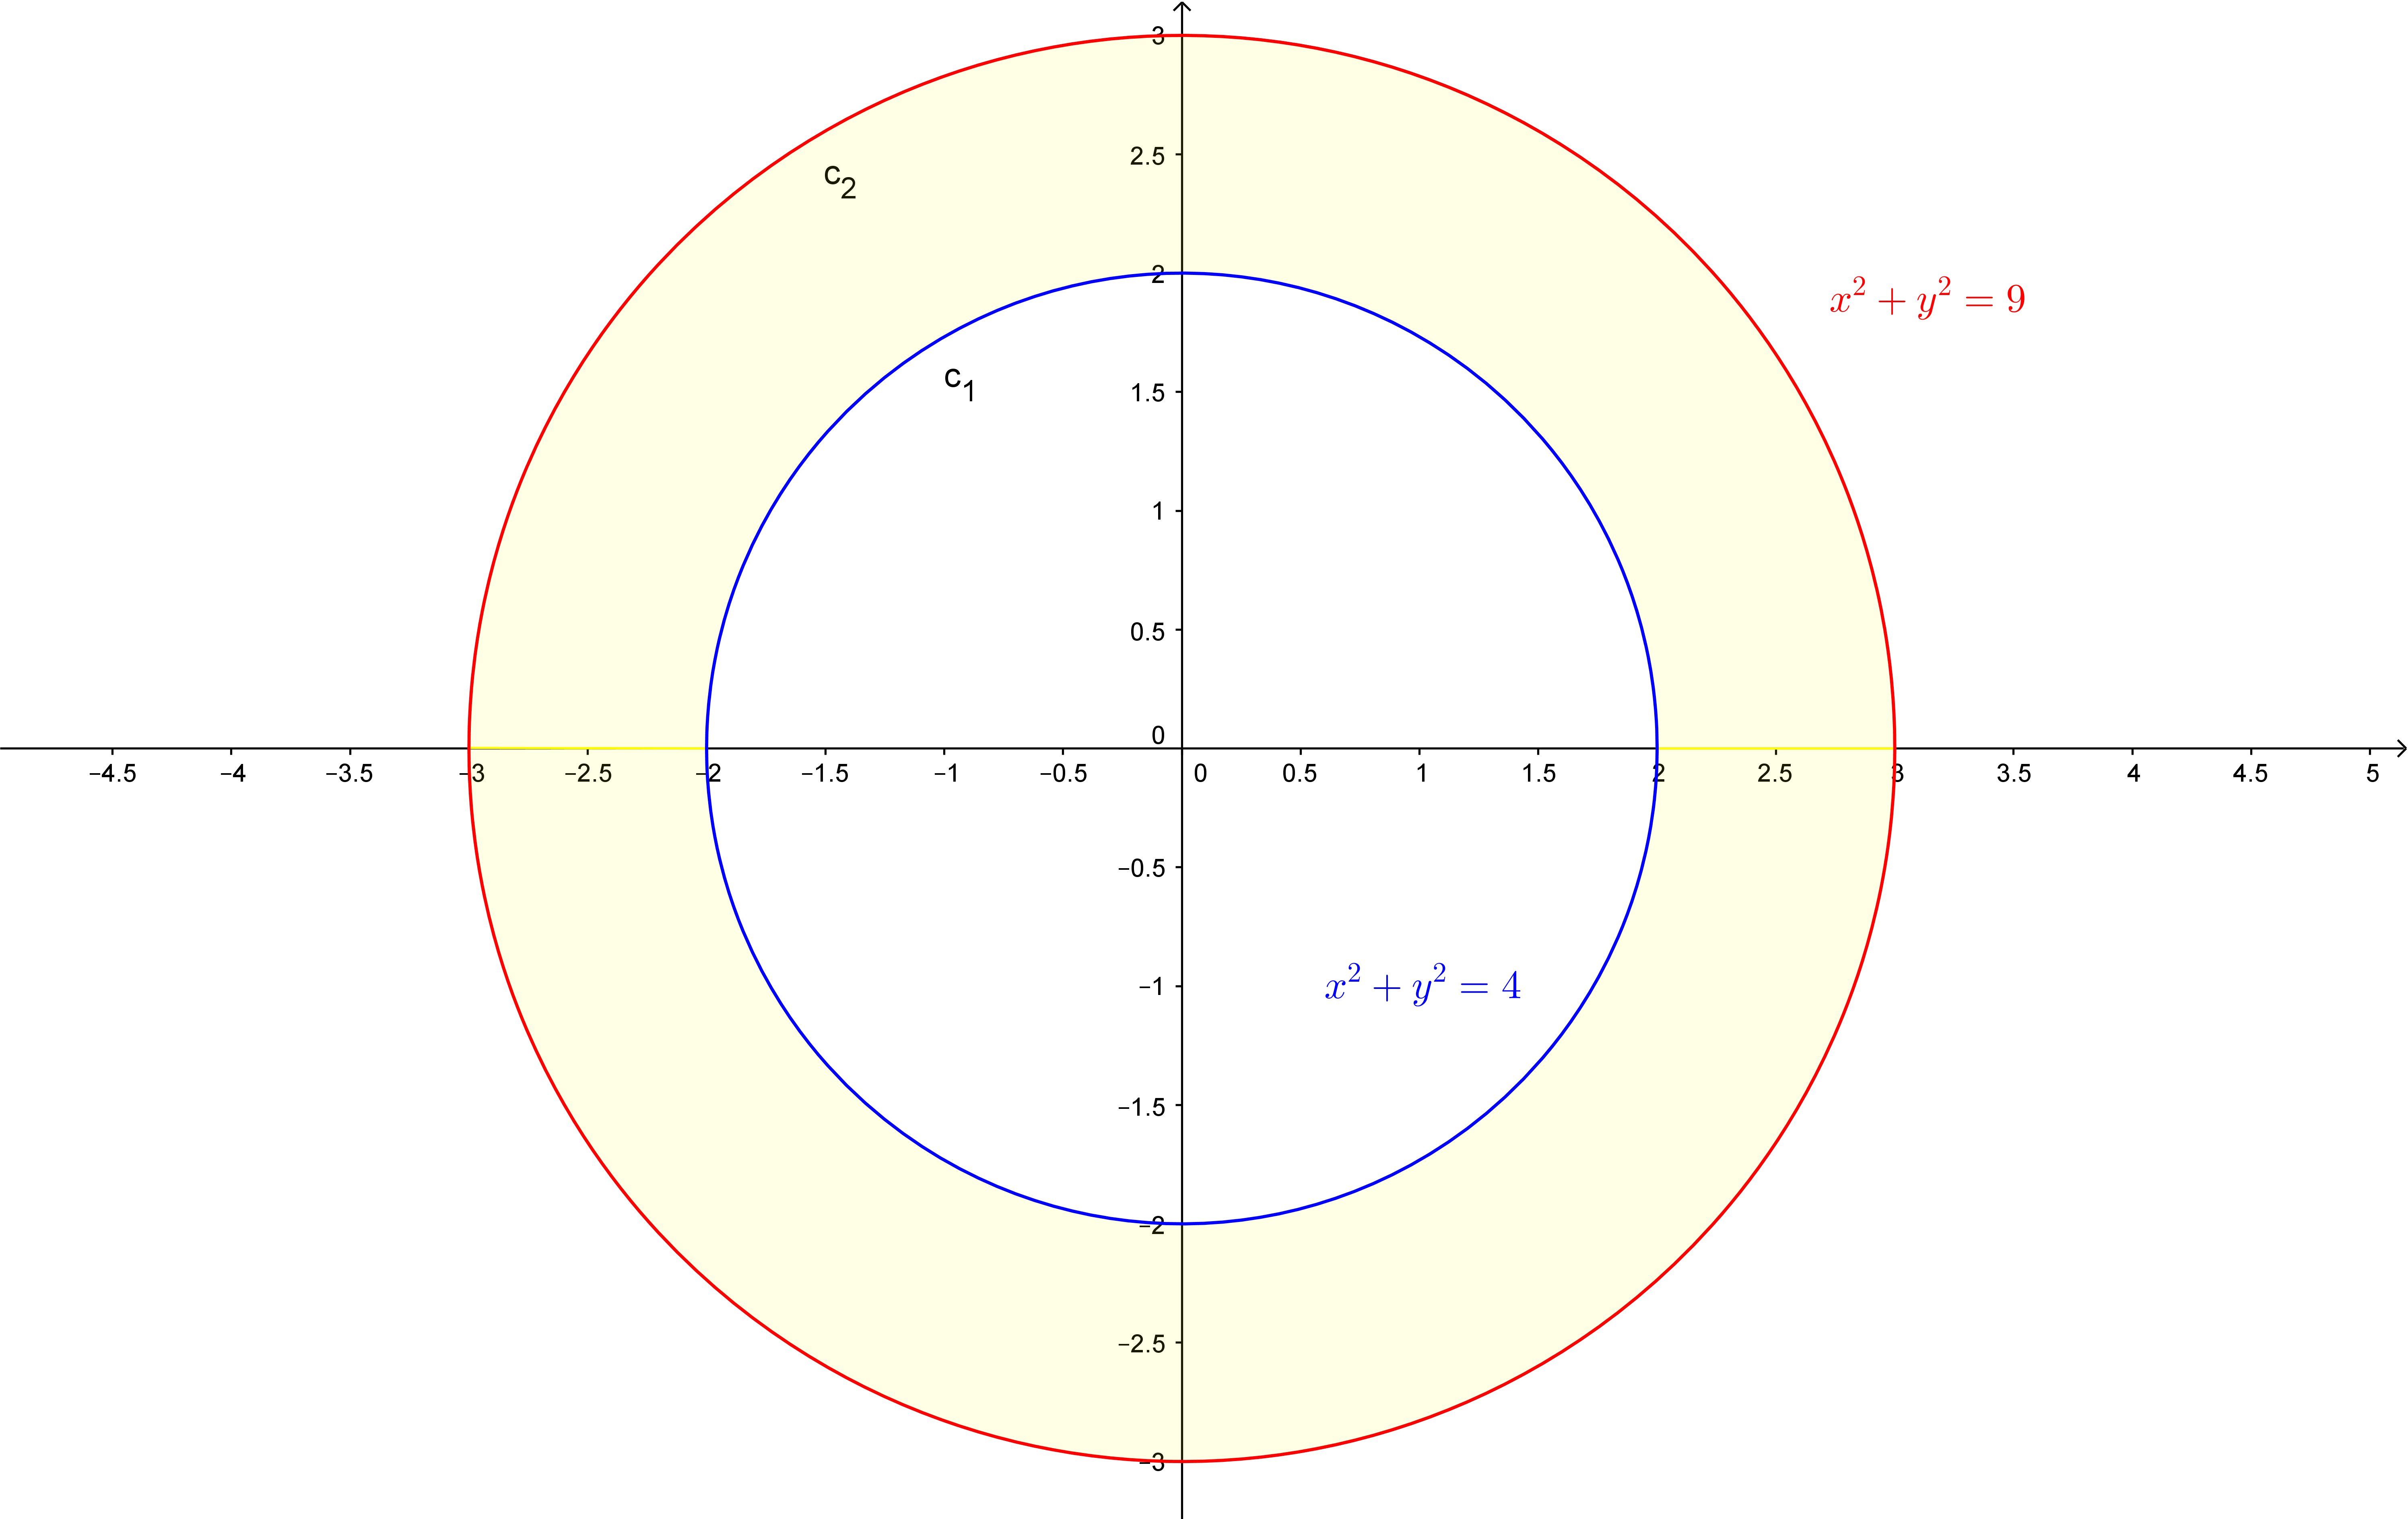
\includegraphics[width=0.5\textwidth]{v12_a02_e01.png}		
	\end{figure}
	
	\begin{equation*}
		x^2 + y^2 = r^2\Rightarrow	\e^{x^2 + y^2} = \e^{r^2}
	\end{equation*}
	\begin{equation*}
		da = dx dy = r\, dr d\theta
	\end{equation*}
	\begin{equation*}
		R = \left\{(r, \theta) \in \mathbb{R}^2 \,|\, 2 \leq r \leq 3,\, 0 \leq \theta \leq 2\pi\right\}
	\end{equation*}		
	\begin{gather*}
		v = \iint_R \e^{x^2 + y^2} dx dy = \int_2^3 \int_0^{2\pi} \e^{r^2} r\, d\theta dr = \int_2^3 \e^{r^2} r\, dr \int_0^{2\pi} d\theta = \int_2^3 \e^u \dfrac{du}{2} \int_0^{2\pi} d\theta =\\ \dfrac{1}{2}\int_2^3 \e^u du \int_0^{2\pi} d\theta = \dfrac{1}{2} \left[\e^u\right]_2^3 [\theta]_0^{2\pi} = \dfrac{1}{\overstrike{2}} \left[\e^{r^2}\right]_2^3 \overstrike{2}\pi = \left(\e^{3^2} - \e^{2^2}\right) \pi = \pi\left(\e^9 - \e^4\right)	
	\end{gather*}
	\begin{equation*}
		u = r^2 \Rightarrow \dfrac{du}{2} = r\, dr
	\end{equation*}
	
	\item Exercício
	
	\begin{equation*}
		\iint_R \sqrt{x^2 + y^2}\, dxdy
	\end{equation*}
	$R$, região cujo o contorno é:
	\begin{equation*}
		x^2 + y^2 = 4
	\end{equation*}
	
	\begin{figure}[htb]
		\caption{Coordenadas polares - Aula 02 - Exercício II}
		\label{v12_a02_e02}
		\centering
		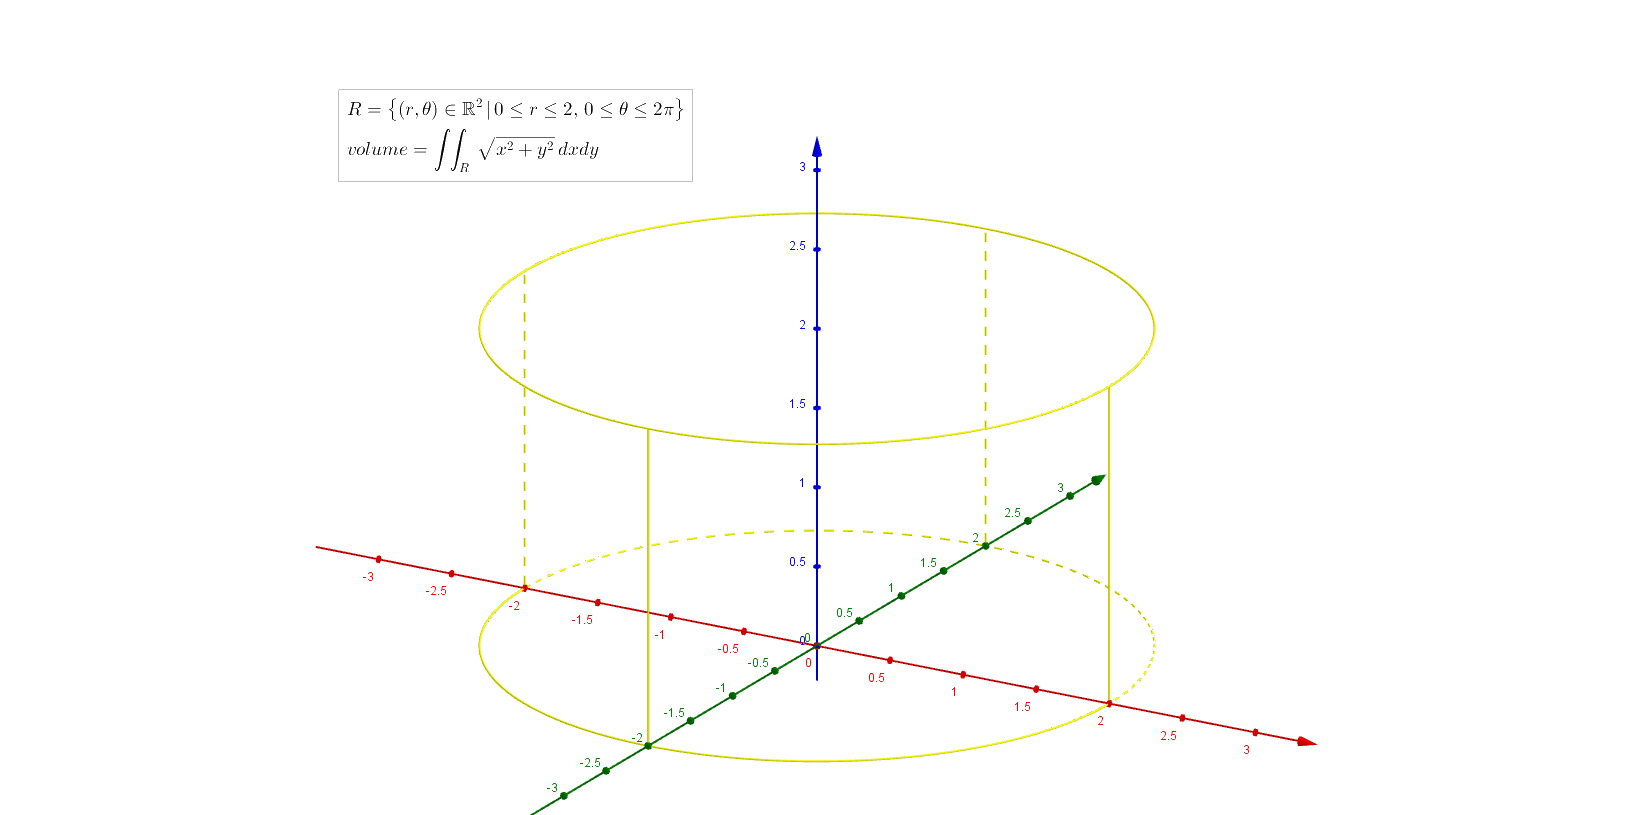
\includegraphics[width=0.5\textwidth]{v12_a02_e02.png}		
	\end{figure}	
	
	\begin{equation*}
		x^2 + y^2 = r^2 \Rightarrow \sqrt{x^2 + y^2} = \sqrt{r^2} = r
	\end{equation*}
	\begin{equation*}
		da = dx dy = r\, dr d\theta
	\end{equation*}
	\begin{equation*}
		R = \left\{(r, \theta) \in \mathbb{R}^2 \,|\, 0 \leq r \leq 2,\, 0 \leq \theta \leq 2\pi\right\}
	\end{equation*}
	\begin{gather*}
		v = \iint_R \sqrt{x^2 + y^2}\, dxdy = \int_0^2 \int_0^{2\pi} r^2\,d\theta dr = \int_0^2 r^2\, dr \int_0^{2\pi} d\theta =\\ \left[\dfrac{r^3}{3}\right]_0^2 [\theta]_0^{2\pi} = \dfrac{2^3}{3}2\pi = \dfrac{16\pi}{3}
	\end{gather*}
\end{enumerate}